\documentclass[a4paper]{article}
\usepackage[warn]{mathtext}
\usepackage[utf8]{inputenc}
\usepackage[T2A]{fontenc}

\usepackage[english,russian]{babel}
\usepackage{multicol}
\usepackage{fancyhdr}
\usepackage{graphicx}
\usepackage{microtype}
\usepackage{wrapfig}
\usepackage{amsmath}
\usepackage{floatflt}
\usepackage{geometry} \geometry{verbose,a4paper,tmargin=2cm,bmargin=2cm,lmargin=1.5cm,rmargin=1.5cm}
\usepackage{float}
\usepackage{amssymb}
\usepackage{caption}
\usepackage{epsfig}
\usepackage{newunicodechar}

\usepackage{xcolor}
\usepackage{hyperref}

\usepackage{listings}
\usepackage{color}
 % Цвета для гиперссылок
\definecolor{linkcolor}{HTML}{799B03} % цвет ссылок
\definecolor{urlcolor}{HTML}{799B03} % цвет гиперссылок
 
\hypersetup{pdfstartview=FitH,  linkcolor=linkcolor,urlcolor=urlcolor, colorlinks=true}

\definecolor{dkgreen}{rgb}{0,0.6,0}
\definecolor{gray}{rgb}{0.5,0.5,0.5}
\definecolor{mauve}{rgb}{0.58,0,0.82}

\lstset{
  language=Java,
  aboveskip=3mm,
  belowskip=3mm,
  showstringspaces=false,
  columns=flexible,
  basicstyle={\small\ttfamily},
  numbers=none,
  numberstyle=\tiny\color{gray},
  keywordstyle=\color{blue},
  commentstyle=\color{dkgreen},
  stringstyle=\color{mauve},
  breaklines=false,
  breakatwhitespace=true,
  tabsize=3
}

\begin{document}

\graphicspath{ {pictures/} }

\begin{titlepage}
	\centering
	\vspace{5cm}
    {\scshape\LARGE NetCracker Learning center\par}
	\vspace{5cm}
	{\scshape\Large  Учебное практическое задание № 1 \par}
	\vspace{1cm}
    {\huge\bfseries  Задание 1. Объектно-ориентированное программиорвание в Java \par}
	\vspace{1cm}
	\vfill
    \begin{flushright}
        {\large выполнил студент}\par
        \vspace{0.3cm}
        {\LARGE Яромир Водзяновский}
    \end{flushright}
	\vfill
Долгопрудный, 2021
% Bottom of the page
\end{titlepage}

\pagestyle{fancy} 
\fancyhead[L]{Java   $\sim  \hat(\, ^{\circ}  \omega  ^{\circ} \, \hat) \sim$}
\fancyhead[R]{NetCracker}
\fancyfoot[C]{ \noindent\rule{\textwidth}{0.4pt} \thepage }



\newpage 


Код лежит на \href{https://github.com/yarvod/NetCracker_LearningCenter/tree/main/Practise_tasks/Practice_task_1}{GitHub}.

\section{Квадратное уравнение}

\textbf{Цель:} Разработайте класс для решения квадратных уравнений. Вычисление дискриминанта должен осуществлять вложенный класс. После компиляции объясните структуру class файлов. Проанализируйте использование вложенного класса. \par


\begin{lstlisting}
    import java.util.Scanner;

    public class Solver {
    
        class Discr {
    
            public double discr_calc(int a, int b, int c) {
                double discr = b*b - 4*a*c;
                return discr;
            }
        }
    
        public static double[] answer(int a, int b, double discr) {
            double[] res = new double[2];
            for (int i=0; i<2; i++) {
                res[i] = (-b + Math.pow(-1, i) * Math.sqrt(discr)) / (2 * a);
            }
            return res;
        }
    
        public static void main(String[] args) {
    
            int[] coeffs;
            double[] answer = new double[2];
    
            Scanner in = new Scanner(System.in);
    
            coeffs = new int [3];
            for (int i=0; i<3; i++) {
                System.out.print("Enter coeff " + i + " : ");
                coeffs[i] = in.nextInt();
            }
            in.close();
    
            int a = coeffs[0];
            int b = coeffs[1];
            int c = coeffs[2];
    
            Solver solver = new Solver();
            Discr discr = solver.new Discr();
    
            double discriminante = discr.discr_calc(a, b, c);
    
            if (a == 0 && b == 0 && c == 0) {
            System.out.println("The Answer: Infinity amount of solutions!");
    
            } else {
                if (discriminante < 0) {
                    System.out.println("The Answer: No solution in Real numbers!");
                } else {
                    if (a == 0) {
                        double answer_linear = -c / b;
                        System.out.println("The Answer: " + answer_linear);
        
                    } if (a == 0 && b == 0 && c != 0) {
                        System.out.println("The Answer: No solution");
        
                    } if (a != 0) {
                    answer = answer(a, b, discriminante);
                    System.out.println("The Answer: " + answer[0] + " and " + answer[1]);
                    }
                }
            } 
        }
    }    
\end{lstlisting}

\begin{figure}[H]
    \begin{center}
        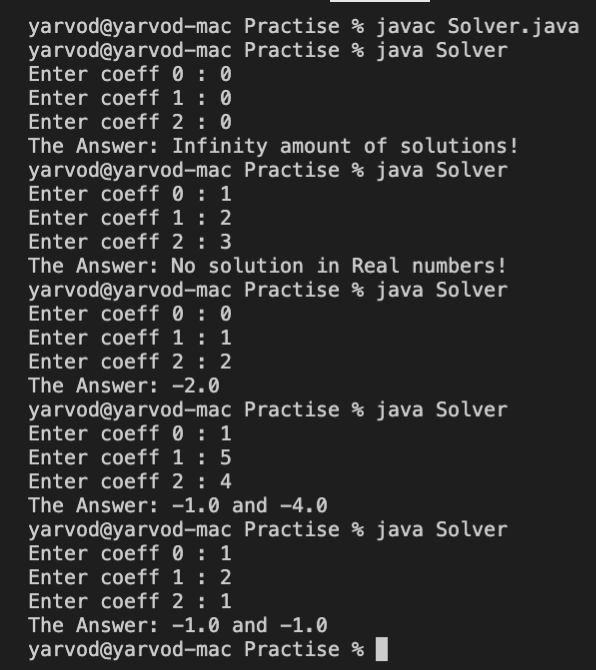
\includegraphics[scale = 0.5]{solution_1.png}
        \caption{Демонастрация работы решателя квадратного уравнения}
        \label{sol_1}
    \end{center}
\end{figure}


\section{Игра в кости}

\textbf{Цель:} Реализуйте игру в кости. Играют N игроков (компьютер в списке последний). Подкидываются одновременно К кубиков. Выигрывает тот, у кого большая сумма очков. Кто выиграл, тот и кидает первым в следующем кону. Игра идет до 7 выигрышей. Начинаете игру Вы. \par 

\begin{lstlisting}
import java.util.Scanner;

public class Game {

    public static int Play(int K) {
        int score = 0;
        for (int j=0; j<K; j++) {
            score += (int) (Math.random() * 6 + 1); 
        }
        return score;  
    }

    public static int[] maxArray(int[] Array) {
        int index = 0;
        int max = 0;
        int[] maxArray = new int[2];
        for (int i = 0; i<Array.length; i++) {
            if (max <= Array[i]) {
                max = Array[i];
                index = i;
            }
        }
        maxArray[0] = index;
        maxArray[1] = max;
        return maxArray;
    }

    public static int[][] Substitute(int[][] PlayerList, int maxScoreIndex) {
        int[] save_winner = PlayerList[maxScoreIndex];
        for (int k=0; k<maxScoreIndex; k++) {
            PlayerList[maxScoreIndex - k] = PlayerList[maxScoreIndex - k-1];
        }
        PlayerList[0] = save_winner;
        return PlayerList;
    }

    public static void main(String[] args) {

        Scanner in  = new Scanner(System.in);
        int N;
        int K;
        int maxScoreIndex;
        
        System.out.print("Enter number of players: ");
        N = in.nextInt();

        System.out.print("Enter number of cubes: ");
        K = in.nextInt();
        in.close();

        int[] Scores = new int[N];
        int[][] PlayerList = new int[N][2];
        int[] TotalScores = new int[N];
        int WinnerIndex = 0;


        for (int i=0; i<N; i++) {
            PlayerList[i][0] = i;
            PlayerList[i][1] = 0;
        }

        for (int round=0; round<7; round++) {

            System.out.println("Round: " + (round+1));
            for (int player_num=0; player_num<N; player_num++) {
                Scores[player_num] = Play(K);
            }
            maxScoreIndex = maxArray(Scores)[0];

            PlayerList[maxScoreIndex][1] += 1;
            
            for (int k=0; k<N; k++) {
                System.out.println("Player " + PlayerList[k][0] + " has score: " + Scores[k]);
            }

            PlayerList = Substitute(PlayerList, maxScoreIndex);
        }

        System.out.println("Outcomes: ");

        for (int k=0; k<N; k++) {
            System.out.println("Player " + PlayerList[k][0] + " has number of victories: " + PlayerList[k][1]);
        }
        
        for (int i=0; i<N; i++) {
            TotalScores[i] = PlayerList[i][1];
        }

        WinnerIndex = maxArray(TotalScores)[0];
        
        System.out.println("Winner of the Game: Player " + PlayerList[WinnerIndex][0]);
    }
}
\end{lstlisting}

\begin{figure}[H]
    \begin{center}
        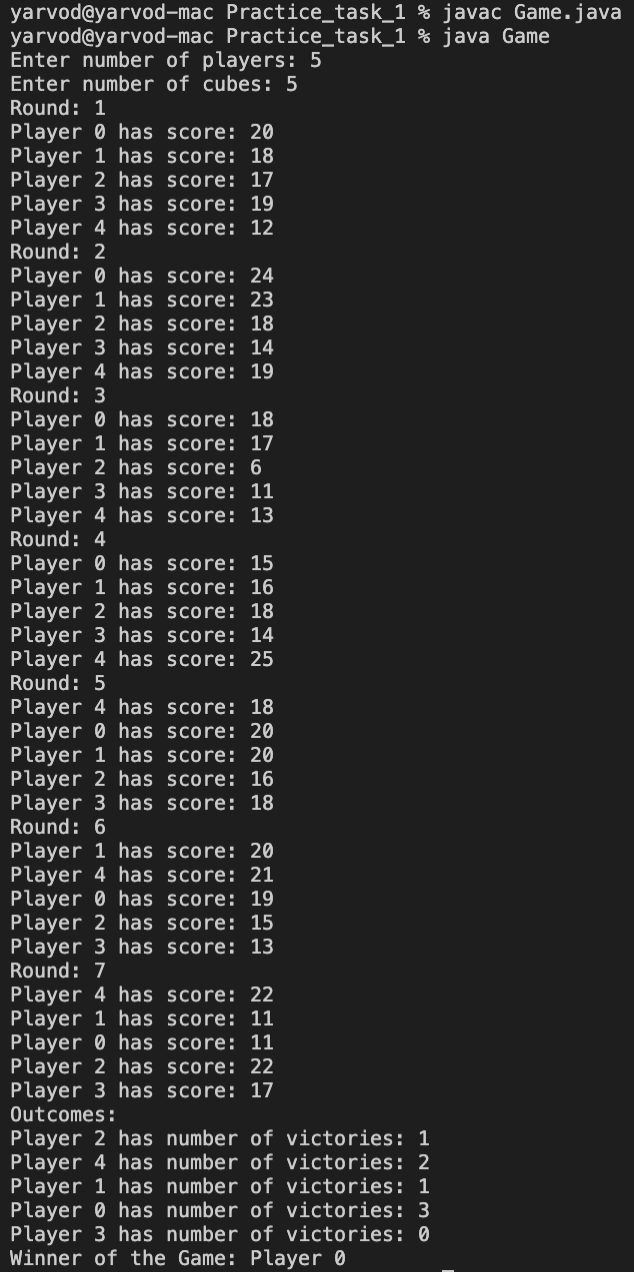
\includegraphics[scale = 0.5]{solution_2.png}
        \caption{Демонстрация работы игры в кости}
        \label{sol_2}
    \end{center}
\end{figure}


\section{Адрес человека}

\textbf{Цель:} Напишите программу «Адрес человека». Есть сущность Человек, которая связана с сущностью Адрес. Считается, что у каждого человека есть только один адрес. Организовать массив объектов Человек (не менее 4) и по массиву:
\begin{itemize}
    \item осуществить поиск Человека по фамилии;
    \item осуществить поиск человека по атрибуту адреса;
    \item вывести людей, родившихся между определенными датами;
    \item найти самого старого (молодого);
    \item найти людей, проживающих на одной улице.
\end{itemize}

\begin{lstlisting}
import java.time.LocalDate;
import java.util.Scanner;

public class HumanAdress {

    class Human {
        String name, surname;
        int age, day_birth, month_birth, year_birth;

        public Human(String name, String surname, int age, int day_birth, int month_birth, int year_birth) {
            this.name = name;
            this.surname = surname;
            this.age = age;
            this.day_birth = day_birth;
            this.month_birth = month_birth;
            this.year_birth = year_birth;
        }

        class Adress {
            int flat, house;
            String street, city, country;
    
            public Adress(int flat, int house, String street, String city, String country) {
                this.flat = flat;
                this.house = house;
                this.street = street;
                this.city = city;
                this.country = country;
            }
        }
    }

    static void print_human(Human human) {
        System.out.println("Human name/surname: " + human.name + " " + human.surname + ", date of birth: " + LocalDate.of(human.year_birth, human.month_birth, human.day_birth));
    }

    static void find_by_surname(String surname, Human[] humans) {
        int k = 0;
        for (int i=0; i<4; i++) {
            if (humans[i].surname == surname) {
                print_human(humans[i]);
                k++;
            }     
        }
        if (k == 0) {
            System.out.println("There is no such person here");
        }
    }

    static void find_age(String args, Human[] humans) {
        int min = 100;
        int max = 0;
        int index = 0;
        if (args == "youngest") {
            for (int i=0; i<4; i++) {
                if (humans[i].age < min) {
                    min = humans[i].age;
                    index = i;
                }
            }
            System.out.print("The youngest: ");
            print_human(humans[index]);
        } if (args == "oldest") {
            for (int i=0; i<4; i++) {
                if (humans[i].age > max) {
                    max = humans[i].age;
                    index = i;
                }
            }
            System.out.print("The oldest: ");
            print_human(humans[index]);
        }
    }


    public static void main(String[] args) {

        HumanAdress human_adress = new HumanAdress();
        Human[] humans = new Human[4];

        humans[0] = human_adress.new Human("Yulya", "Prokhorova", 20, 11, 7, 2001);
        humans[1] = human_adress.new Human("Artem", "Atepalikhin", 21, 29, 4, 2000);
        humans[2] = human_adress.new Human("Alexandrov", "Alexandr", 16, 20, 4, 2005);
        humans[3] = human_adress.new Human("Diana", "Chikan", 19, 4, 8, 2001);

        System.out.print("Enter a surname to find: ");
        Scanner in  = new Scanner(System.in);
        String entered_surname = in.next();
 
        find_by_surname(entered_surname, humans);

        System.out.println("youngest or oldest human you want to know? ");
        String entered_answer = in.next();
        find_age(entered_answer, humans);

        in.close();
    }
}

\end{lstlisting}




\end{document}